\documentclass[11pt]{article}

\usepackage{chngcntr}
\usepackage[italian]{babel}
\usepackage{amsmath}
\usepackage{amssymb}
\usepackage[margin=1in]{geometry}
\usepackage[utf8]{inputenc}
\counterwithin*{section}{part}
\usepackage{enumitem}
\usepackage[autostyle]{csquotes}
\usepackage{array}
\usepackage{multirow}
\usepackage{graphicx}

\graphicspath{ {./img/} }


\newenvironment{nosepitemize}{\begin{itemize}[noitemsep,topsep=0ex]}{\end{itemize}}


% email: (@unimib.it o @jakala.com)
% nico.didomenica@unimib.it
% attilio.revivo@unimib.it
% tutor data science: giovanni.collini@unimib,it
% tutor per gli altri: marta.laudiano@unimib.it

\title{\textbf{Web Marketing and Communication Management}}
\author{}
\date{}


\begin{document}
\maketitle
\begin{abstract}
  Per i frequentanti l'esame consisterà in un progetto che farà media con lo scritto, con possibilità di orale integrativo.
  Il progetto (fatto in gruppi di tre persone) per Data Science sarà un progetto in R di elaborazione dei dati con relativa presentazione.
  Altrimenti, per le altre facoltà, l'esame consiste in una presentazione frontend e backend di un'app (pre-esistente) proposta da un cliente.
  Per il corso di DataScience inoltre vi saranno delle lezioni di tutorato su R.
  
  Per i non frequentanti l'esame consiste in uno scritto (composto da 10 domande aperte) e un orale.
  L'esame comunque verte solamente sulle slide.
\end{abstract}

\section{Lezione 1 - Attilio - 01 marzo}
% @momolo {{{
% mi spiace ragazzi, vado a fare foundation of probability...
% se volete continuare la dispensa avete tutta la mia stima :)
% }}}
Diverse definizioni di marketing:
\begin{enumerate}[noitemsep,topsep=0ex]
	\item Consiste nell'individuazione e nel soddisfacimento dei bisogni umani e sociali. 
	Il marketing è soprattutto una prospettiva.
	Non si parla, in questa fase, di soldi e di profitti (che però sono sottintesi). 
	L'accezione risulta più filosofica, c'è una sorta di attenzione verso il prossimo.
	
	\item (AMA - American Marketing Association): Il marketing è l'insieme di attività, istituzioni (c'è anche un elemento personale, nel senso che ci sono delle persone che fanno marketing) e processi volti alla creazione, alla comunicazione e allo scambio di offerte (se c'è un bisogno che non è ancora espresso, bisogna anche pensare ai prodotti non esistenti e quindi alla creazione; ma una volta creato è importante anche comunicarlo e scambiarlo) che hanno valore per acquirenti, clienti, partner e per la società in generale (e cioè sono coinvolte un gran numero di persone). 
	E' una definizione più tecnica e calata nella realtà rispetto alla prima.
	
	\item L'insieme dei processi, coerenti e coordinati, finalizzato a produrre scambi e relazioni, fra individui e organizzazioni, con una finalità sempre duplice: 
	\begin{itemize}[noitemsep]
		\item creare valore economico e sociale per l'offerta;
		\item trasferire valore funzionale, simbolico, emozionale o esperienziale per la domanda.
	\end{itemize} 
	Qui si accenna il tema della funzione sociale. 
	Si vogliono soddisfare dei beni non sempre tangibili, quindi oltre il mangiare e/o il bere.
	
	\item Una visione sociale: Il marketing è il processo sociale mediante il quale individui e gruppi ottengono ciò di cui hanno bisogno e ciò che desiderano tramite la creazione dell'offerta e il libero scambio di prodotti e servizi di valore.
\end{enumerate}

~\\
Un'affermazione di Peter Drucker che spiega molto bene il marketing: 
\enquote{Si può sempre presumere che vi sarà sempre necessità di vendere.
	Ma lo scopo del marketing è  quello di rendere superflua la vendita. 
	Lo scopo è conoscere e comprendere il cliente al punto che il prodotto o servizio sia tanto adatto alle sue esigenze da vendersi da solo.
	Teoricamente il risultato del marketing è un cliente pronto a effettuare l'acquisto. 
	Allora non rimane che rendere disponibile il prodotto o servizio.}
\newline
Con questa definizione si osserva che l'operazione di vendita è separata dal marketing. L'obiettivo è conoscere le persone che hanno determinati bisogni e trovare il modo di soddisfarli. Ad esempio, vendere ghiaccio agli Eschimesi non significa fare marketing ma solamente essere bravo a vendere un prodotto.

\noindent
Due prospettive complementari del marketing:\\

\begin{center}
	\begin{tabular}{c | c}
		Analisi di marketing & Marketing management \\
		\hline
		\begin{tabular}{l}
			\\
			BtoC (Business to Consumer) \\
			BtoB (Business to Business) \\
			CtoC (Consumer to Consumer)\\
			BtoG (Business to Government)\\
		\end{tabular}
		
		&
		
		\multicolumn{1}{m{9cm}}{~\newline Ovvero l'arte e la scienza della scelta dei mercati obiettivo, nonché dell'acquisizione, del mantenimento e della crescita della clientela tramite la creazione, la distribuzione e la comunicazione di un valore superiore}
	\end{tabular}
\end{center}

\noindent
I campi d'azione del marketing sono:
\begin{itemize}[noitemsep,topsep=0ex]
	\item Beni
	\item Servizi
	\item Eventi
	\item Esperienze: ad esempio Eataly
	\item Persone: uno che tifa una squadra come Inter (preferenze personali)
	\item Luoghi: Turista
	\item Diritti di proprietà: Disney lascia usare il topolino sulla maglietta di altri
	\item Organizzazioni
	\item Informazioni: Tante aziende fanno marketing su quanto sono brave a raccogliere, gestire e sfruttare le informazioni
	\item Idee: ha a che fare con la comunicazione sociale
\end{itemize}
~\\
Gli attori del marketing sono:
\begin{itemize}[noitemsep,topsep=0ex]
	\item Marketing manager che è responsabile della gestione della domanda;
	\item Il cliente potenziale che ormai ha un ruolo sempre meno passivo, cosa che rende il marketing un po' più complesso per le aziende.
\end{itemize}
~\\
Gli stati della domanda sono:
\begin{itemize}[noitemsep,topsep=0ex]
	\item Domanda negativa: Una cosa che non ti piace e che non riesci proprio a vedere, ad esempio l'olio di palma;
	\item Domanda inesistente: è una domanda non esistente perché non interessa a nessuno;
	\item Domanda latente: è un domanda esistente ma non c'è nessuno che la produce. E' il paradiso per un marketing manager. Ad esempio, il primo Mac contro quello di IBM (grande ingombrante) oppure gli smartphone con le loro fotocamere.
	\item Domanda declinante;
	\item Domanda irregolare;
	\item Domanda piena;
	\item Domanda eccessiva;
	\item Domanda nociva: un esempio può essere dato dalle sigarette
\end{itemize}
\noindent
La domanda è essenziale per definire il mercato, senza questa non esisterebbe il marketing.
Secondo gli economisti è un insieme di acquirenti e venditori che effettuano transazioni su un prodotto o un insieme di prodotti.
Tradizionalmente era il luogo fisico dello scambio dei beni e servizi. 
Oggi è molto più de-localizzato, basti vedere Amazon come esempio.
Secondo i marketing manager il mercato è costituito da un gruppo di clienti differenti sulla base dei loro bisogni, prodotti, geografia e demografia. I venditori si raggruppano in settori. 
~\\

\noindent Un semplice sistema di marketing è:
\begin{verbatim}
                     ----->[Comunicazioni]---->-->
                    |                            |
                 Settori   ---[Beni/Servizi]--> Mercato
                (insieme di                    (insieme di
                venditori)  <----[Denaro]-----  aquirenti)
                    |                            |
                    <--<----[Informazioni]<------
\end{verbatim}

\noindent I diversi tipi dei mercati sono:
\begin{itemize}[noitemsep, topsep=0ex]
	\item Mercati dei consumatori o di consumo
	\item Mercati delle imprese
	\item Mercati globali
	\item Mercati delle organizzazione non-profit
	\item Mercati della pubblica amministrazione
\end{itemize}

\noindent
I mercati oggi sono sempre più globali; il mercato locale, ad esempio, dipende anche da quello che succede in Cina. 
Il marketplace è il luogo (fisico o virtuale) dove avvengono le transazioni.
Il marketspace è lo spazio di mercato.
Il meta-mercato nasce da un'idea di Mohan Sawhney e indica un insieme dei prodotti complementari e strettamente correlati nella mente dei consumatori, anche se situati in settori distinti. Ad esempio, nell'ambito del turismo uno può voler andare in un Luna Park o al cinema oppure preferisce stare in un campeggio o in un hotel a 5$\star$.

Bisogna essere bravi a individuare il proprio mercato di riferimento: è essenziale per costruire strategie interessanti, ma anche per reagire a eventuali cali nelle vendite.
~\\

\noindent I concetti chiave del marketing: 
\begin{itemize}[topsep=0ex] %meglio non usare noitemsep
	\item Bisogni, desideri e domanda
	\begin{itemize}[topsep=0ex,noitemsep]
		\item Per i bisogni si segue la gerarchia dei bisogni di Maslow:
		
		1. Bisogni Fisiologici $\to$ 2. Bisogni di Sicurezza 
		$\to$ 3. Bisogni Sociale $\to$ 4. Bisogni di Stima $\to$
		5. Bisogni di auto-realizzazione.
		
		%Inoltre i bisogni possono essere di diverso tipo: Bisogni Espressi, Reali, Inespressi, di Gratificazione e Segreti.
		\item I desideri sono plasmati in funzione della cultura, della società e della psicologia
		\item la domanda è un desiderio specifico insieme alla capacità (economica o pratica) di soddisfarlo
	\end{itemize}
	
	\item La piramide di Maslow
	
	Cinque livelli di bisogni: è inutile che propongo il soddisfacimento dei bisogni del quarto livello se non ho soddisfatto i bisogni del primo, secondo o terzo livello.
	
	Risulta interessante sapere il livello di bisogno del mercato a cui si fa riferimento. Se si riuscisse a salire di livello facilmente, il gioco si farebbe interessante: più si sale e più ci si allontana dalla soddisfazione dei bisogni primari, e quindi dalla gente povera.
	
	Il sogno di tutti i marketer sarebbe arrivare facilmente in cima, ma non è possibile soddisfare i bisogni dei livelli alti senza essersi occupati prima di quelli alla base.
	
	\item Mercati obiettivo, posizionamento e segmentazione:
	
	Non tutti i consumatori sono uguali, quindi è importante suddividere il mercato in segmenti e definire quali segmenti siano prioritari in termini di opportunità; questo tipo di mercato è detto di tipo obiettivo. A ogni mercato obiettivo viene dedicata un'offerta specifica, che poi viene posizionata nella mente dei potenziali clienti evidenziando i vantaggi distintivi rispetto agli altri.
	\item Offerte e marche:
	
	Le imprese rispondono ai bisogni dei clienti definendo una proposta di valore (value proposition), ossia un insieme di benefici atto a soddisfare tali bisogni. La value proposition può essere tangibile (costo, assistenza) o intangibile. La value proposition diventa concreta in un'offerta. La marca è un'offerta proveniente da una fonte nota, conosciuta, a cui vengono associati elementi caratterizzanti.
	\item Valore e soddisfazione:
	
	L'acquirente sceglie le offerte che gli forniscono il maggior Valore, che altro non è che il rapporto tra benefici e costi (tangibili o intangibili). L'intangibilità rende la formula incerta quindi deve essere identificata e/o creata. \newline
	In tal senso il marketing management è l'attività che identifica, crea, comunica, distribuisce, misura e controlla il valore per il cliente.\newline
	La soddisfazione è il frutto del percepito rispetto alle aspettative.
	\item Canali e marketing:
	\begin{itemize}[noitemsep,topsep=0ex]
		\item Canali di comunicazione: il canale che l'azienda usa, una volta era a una via, adesso a due vie, per dare informazioni, offerte ecc. Ce ne sono tantissimi: la pubblicità, la mail, i Social.
		\item Canali di distribuzione: Solitamente negozi, Internet sta diventando un grande canali di distribuzione ed è anche un canale di comunicazione.
		\item Canali di servizio: Helpdesk, assistenza clienti.
		
		I tre canali possono essere sovrapposti, ad esempio Internet può essere usato anche come canale di servizio attraverso l'uso di Twitter.
	\end{itemize}
	\item Supply chain:
	
	E' il canale che va dalle materie prime fino ai prodotti finiti. 
	Il sistema di distribuzione della supply chain fa riferimento a più aziende/operatori che si suddividono il valore totale.
	Alcune aziende usano strategie di integrazione verticale, acquisendo le catene intermedie, per acquisire una quota maggiore di tale valore.
	\item Concorrenza:
	
	La concorrenza comprende tutte le offerte che possono essere considerate da un acquirente come un'alternativa possibile per la soddisfazione di un dato bisogno. I concorrenti possono essere palesi o totalmente inaspettati e insospettabili.
	Se 15 anni fa avessero detto alla Kodak che i concorrenti sarebbero stati Apple e Samsung, i vertici di Kodak si sarebbero messi a ridere. Però il mondo è cambiato e la fotografia da cellulare ha spazzato via il mondo dei rullini su cui Kodak aveva un'egemonia pressoché assoluta.\newline
	Per un'attività di successo è cruciale identificare con precisione il perimetro della concorrenza. Chi non accetta il cambiamento, inoltre, muore.
	\item Ambiente di marketing
\end{itemize}

\bigskip
\noindent I fattori che influenzano l'evoluzione del marketing:
\begin{itemize}[noitemsep, topsep=0ex]
	\item Tecnologia di rete

		\quad Oggi abbiamo un potenziale tecnologico molto elevato. Fino a qualche anno fa alcune pratiche erano ancora sconosciute.
	
	\item Globalizzazione
	
		\quad Buona o meno, dipende dal punto di vista. Tuttavia rimane un dato di fatto: si può comprare qualsiasi cosa in qualsiasi posto del mondo, portando anche a risparmi evidenti.
			
	\item Deregolamentazione
	
		\quad Tendenzialmente in tutto quello che facciamo le regole contano sempre di più, ma bisogna tenere conto delle regole vigenti in tutti gli altri paesi, e non solo delle proprie.
Ogni decisione impatta sui mercati, sia che questa venga dall’interno, sia che venga dall’esterno.
	
	\item Privatizzazione
	\item Livello di concorrenza più elevato
	
		\quad Si creano inevitabilmente molti più competitor, dovuti al fatto che tutti possono fare tutto e con costi meno elevati a causa delle tecnologie di rete.
	
	\item Convergenza di settore
	
		\quad Il caso Kodak e Apple/Samsung rende bene l’idea.
Con il car sharing cambia la fisionomia dei mercati, il possesso diventa secondario.
	
	\item Trasformazione del commercio al dettaglio
	
		\quad In Italia abbiamo ancora moltissimo negozi al dettaglio, negli altri paesi sono già quasi tutti scomparsi.
Dal punto di vista economico, non ha senso rivolgersi a questi negozietti.
Correlata alla globalizzazione.
	
	\item Disintermediazione
	
		\quad Correlato alla globalizzazione anche questo punto.
Non serve più il professore: se programmi bene una macchina, questa può fare il compito del professore, non peggio di come lo farebbe lui. (ex.: professore indiano che ha lasciato un pc con sopra un corso di fisica nucleare in un villaggio indiano, in mano a dei bambini)
	
	\item Potere d'acquisto dei consumatori
	
		\quad I prezzi si abbassano a causa della aumentata concorrenza, quindi il potere d'acquisto aumenta.
Risulta anche una capacità di capire meglio le cose.
	
	\item Informazione dei consumatore
	
		\quad Oggi, se si è un minimo attenti, si può sapere molto e molto meglio rispetto al passato sul mondo che ci circonda. Risulta davvero difficile abbindolare il prossimo con campagne marketing massicce.
	
	\item Partecipazione dei consumatori
	
		\quad Il consumatore può partecipare di più, sia in termini positivi che negativi.
Rende il processo più maturo e consapevole. Basti pensare alle polemiche che nascono, ai commenti negativi sui Social. Tutti segnali di una partecipazione attiva.
	
	\item Resistenza dei consumatori
	
		\quad Un consumatore dovrebbe essere attento e un filo più impermeabile alle bufale e alle truffe riscontrabili su internet.
	
\end{itemize}
~\\
\noindent In parallelo i marketing manager possono:
\begin{itemize}[noitemsep,topsep=0ex]
	\item Utilizzare Internet come potente canale informativo e di vendita
	\item Ottenere informazioni più complete e approfondite sui mercati, clienti acquisiti, clienti potenziali e concorrenti
	\item Entrare nei social media per amplificare il messaggio e la comunicazione esterna
	\item Inviare pubblicità/promozioni/campioni a clienti che lo hanno richiesto/consentito
	\item Raggiungere i consumatori in movimento (sfruttando mobile marketing)
	\item Produrre/vendere beni differenziati a livello individuale
	\item Migliorare la propria organizzazione
	\item Migliorare l'efficienza
\end{itemize}
~\\
Il marketing olistico è costituito da diverse componenti:
\begin{verbatim}
Funzione     Alta      Altre Funzioni    Comunicazioni   Prodotto e    Canali
Marketing  Direzione    Aziendali                    \    Servizi       /
     \        |           /                           \      |         /
      \       |          /                             \     |        /
       \      |         /                               \    |       /
        \     |        /                                 \   |      /
        Marketing Interno                             Marketing Integrato
                        \                            /
                         \                          /                           
                          \                        /
                           \                      /
                            \                    /
                              Marketing Olistico 
                            /                    \
                           /                      \
                          /                        \
                         /                          \
            Marketing   /                         Marketing Relazionale
       Socialmente Responsabile                       /      |     \
       /    |       |     \                          /       |      \
      /     |       |      \                        /        |       \
  Etica  Ambiente  Sistema  Comunità             Clienti    Canali     Partner
                   Legale                                                            
\end{verbatim}

Il marketing relazionale ha lo scopo di costituire relazioni a lungo termine, con reciproca soddisfazione delle parti in causa, in modo da migliorare e sviluppare le rispettive attività economiche. 
Le categorie di soggetti sono: Clienti, Dipendenti, Partner di marketing e Membri della comunità finanziaria dell'impresa. 

Attirare un nuovo cliente può costare 5 volte di più di quanto costi sviluppare una relazione con i clienti già acquisiti. Inoltre al concetto di share of market si affianca il concetto di share of customer e la sua crescita passa attraverso cross-selling (ex.: ti ho venduto il cellulare ti vendo anche le cuffiette), up-selling (ti ho venduto 10 bottiglie e ora te ne vendo 20) e trading-up (ha comprato la bottiglia a 50 unità e adesso compra la bottiglia a 75 unità, decido di fare un upgrade di qualità nonostante il prezzo aumenti). 

Si parla del mercato integrato quando vengono progettate e realizzate attività di marketing finalizzate a comunicare e trasferire valore ai clienti in modo che l'intero sia maggiore della somma delle sue parti. 
Per fare ciò occorre mappare le diverse attività di marketing e poi progettare e realizzare ogni singola attività tenendo conto di tutte le altre, in modo che, opportunamente integrate, rendano massimo il valore per il cliente.

Nel marketing olistico, i dipendenti dell'azienda sono anch'essi parte del processo di marketing e contribuiscono al successo dei piani aziendali. 
E' opportuno dedicare tempo e risorse per allineare il personale a quanto l'azienda propone all'esterno. Questo viene gestito con il marketing interno.

Il performance marketing richiede la comprensione dei ritorni finanziari e non dei programmi di marketing in una prospettiva ampia. 
E' opportuno monitorare un sistema articolato di indicatore(ricavi, soddisfazione dei clienti, aspetti legali, etici, sociali ed ambientali). 
Inoltre è sempre più rivelante la responsabilità finanziaria ossia la capacità di valutare l'impatto finanziario di un piano di marketing attraverso metriche sempre più complesse ed articolate.

\section{Lezione 1 - Di Domenica - 13 marzo} 
\textbf{Customer Experience}(CRM) è come l'azienda interagisce con il cliente. Prima le aziende si concentravano di più sul prodotto che sul cliente adesso invece si concentrano tanto sul cliente e il prodotto viene influenzato dal cliente. Infatti si può vedere che il 50\% dei clienti hanno aspettative più alte rispetto al passato e il 70\% è estremamente frustrato dalle promesse non mantenute. Inoltre abbiamo che un cliente soddisfatto condivide la sua esperienza con 4/5 persone mediamente mentre un cliente insoddisfatto lo fanno con 9/12 persone.

Framework per la Customer Experience:

Monitorare l'esperienza durante l'intero ciclo di vita del cliente, che consiste nel conoscere, considerare, comparare, comprare e infine possedere,  attraverso tutti i canali di contatto tra cui:
\begin{itemize}[noitemsep,topsep=0ex]
	\item Negozio/Assistente di vendita
	\item TV, Radio, Outdoor
	\item Direct mail (posta)
	\item E-mail
	\item Telefono/Cellulare
	\item Web/Portale
	\item Blog/Social
	\item Influenza sociale
\end{itemize}
Dopo aver utilizzato questi canali bisogna introdurre un circolo virtuoso basato sulla conoscenza ed il valore del cliente:
\begin{verbatim}
Comprendere(Data Analytics)------>Valorizzare(Consigli per far 
         >                                    sentire il cliente bene)
         |                                      |
         |                                      |
         |                                      |
         |                                      <
Monitorare(con il reporting)<-----Engage(Classici piani 
                                         fedeltà o premi)
\end{verbatim}
Infine devo allineare i processi organizzativi relativi alla Customer Experience, quindi devo gestire l'organizzazione, i sistemi e il processo.

Posso avere 3 driver che mi rendono la comunicazione con il cliente più efficace (clusterizzare i cliente):
\begin{enumerate}[noitemsep,topsep=0ex]
	\item Per comportamento d'acquisto, per tracciare e collegare le transazioni al cliente. Una volta capito il tipo di transazioni usate si possono identificare 3 macrogrupppi:
	\begin{itemize}[noitemsep,topsep=0ex]
		\item Tradizionale
		\item Multi-Channel
		\item Tech-Advocate
	\end{itemize}
	\item Per esigenza, si divide in 3 gruppi:
	\begin{itemize}[noitemsep,topsep=0ex]
		\item Famiglia 
		\item Giovane coppia
		\item Single
	\end{itemize}
	\item Per valore, posso scoprire chi è:
	\begin{itemize}[noitemsep,topsep=0ex]
		\item Fedele
		\item Alto Spendente 
		\item Basso Spendente
	\end{itemize}
\end{enumerate}
Una volta clusterizzato/caratterizzato il cliente, ci parlo con i vari canali di comunicazione. Infine c'è la customer journey: 
\begin{itemize}[noitemsep,topsep=0ex]
	\item Awareness: devo farmi conoscere;
	\item Knowledge: come mi conoscono gli altri e come mi relaziono; 
	\item Consideration: come il cliente mi considera; 
	\item Selection: il cliente mi sceglie/seleziona;
	\item Satisfaction: il cliente è soddisfatto e torna altre volte da me; 
	\item Loyalty: uso degli acceleratori che mi permettono di agganciare il cliente;
	\item Advocacy: i miei clienti diventano i miei messaggeri.
\end{itemize}

Tutto questo è possibile grazie all'analisi dei dati che comprende: Raccolta dati dei clienti e potenziali clienti, poi interviene la gestione di tali dati(Data Management) nella quale vengono Puliti, Deduplicati e Normalizzati questi dati. Tra i punti principali della gestione dei dati abbiamo Mater Data che serve sopratutto per intercettare inserimento dei dati duplicati e la Privacy. 
Poi abbiamo la fase di Analisi dei dati e Machine Learning per la segmentazione dei clienti (cluser analysis), insights e reporting da cui traiamo le strategie per marketing, merchandising e retailing. 
Infine abbiamo le operations che consistono nella la pianificazione e design della campagna e la sua esecuzione da cui si traggono altri dati, ri-iniziando così il circolo.

Con la gestione virtuosa della Customer Experience abbiamo diversi benefici:
\begin{itemize}[topsep=0ex,noitemsep]
	\item Increme to della loyalty: 
	I clienti rimangono con l'azienda più a lungo e tendono ad essere più fedeli e soddisfatti se il servizio offerto si adatta meglio alle loro esigenze;
	\item Incremento opportunità di vendita: 
	Le aziende che gestiscono meglio la customer experience hanno alto indice di up/cross selling;
	\item Riduzione dei costi: 
	Aumenta l'efficienza nell'erogazione del servizio, inoltre si ha una riduzione della attrition e costi di retention, si riducono anche i costi del marketing, vendita e post-vendita;
	\item Incremento advocacy: 
	I clienti soddisfatti raccomandano i prodotti/servizi dell'azienda e richiedono meno frequentemente servizi ed attenzione(visto che sono soddisfatti della qualità del prodotto).
\end{itemize}

%importante ha  detto che lo chiede all'esame in qualche appello.
Customer Journey ha 3 macroaree:
\begin{enumerate}[noitemsep,topsep=0ex]
	\item Prima dell'acquisto: può riguardare un prospect (potenziale cliente) o un customer, prima dell'acquisto posso fare
	\begin{itemize}[noitemsep,topsep=0ex]
		\item Passaparola (Canale umano);
		\item Vetrina (Canale Fisico);
		\item Cartellonistica (Canale Fisico);
		\item Catalogo (Canale Fisico);
		\item Rivista Digitale (Canale Digitale);
		\item Website (Canale Digitale);
		\item Testimonial e Celebrità (Canale Umano o Digitale);
		\item Social (Canale Digitale).
	\end{itemize}
	Per farmi crescere come marchio, per farmi conoscere, per essere attraente.
	
	\item Durante l'acquisto: Uno volta che mi sono fatto conoscere e il cliente entra nel negozio, entrano in gioco:
	\begin{itemize}[noitemsep,topsep=0ex]
		\item Promotors che propongono i prodotti oppure le offerte ai clienti (Canali Umano); 
		\item Design e Layout dello Store (Canale Fisico); 
		\item E-commerce (Canale Digitale); 
		\item Assistente di vendita opportunamente formate (Canale Umano);
		\item Icone del marchio ovver le immagini associati al marchio come il colore, logo (Canale Fisico);
		\item Iterazione con il prodotto (Canale Fisico).
	\end{itemize} 
	
	\item Dopo l'acquisto per tenere stretto il cliente l'azienda può usare: 
	\begin{itemize}[noitemsep,topsep=0ex]
		\item Promozioni Dedicate (Canale Fisico); 
		\item Eventi, proponendo nuove esperienze ai clienti più fedeli (Canale Fisico); 
		\item Newsletter e Mailing, per dire come si sta evolvendo l'azienda e i nuovi prodotti che ha (Canale Digitale);
		\item Call Center in realtà costa tanto quindi tante aziende stanno iniziando a sfruttare dei bot che rispondono alle domande più comuni (Canale Digitale);
		\item Social Network Aggiorno il cliente, faccio pubblicità (Canale Digitale); 
		\item Post-Vendita, ti seguo dopo la vendita, chiedendo magari il feedback sul prodotto (Canale Fisico o Digitale).
	\end{itemize}
\end{enumerate}



\section{Lezione 2 - Di Domenica - 15 marzo} %Di Nico

Nella Strategia della customer experience abbiamo: la \textbf{Contact Strategy}, va a braccetto con la \textbf{Contact Policy}, in realtà in alcune aree vanno in contrapposizione. La comtact strategy comprende:
\begin{itemize}[noitemsep,topsep=0ex]
	\item Chi vado a contattare(quali sono i target) e come vado a contattarli. 
	\item Una volta definito il target devo definire gli obbiettivi della campagna, le campagne possono essere di ingaggio oppure di soddisfazione (quali campagne creano soddisfazione al cliente). 
	\item Poi arriva il mezzo (come): posso usare le porte analitiche o quelle tecnologiche.
	\item Infine è fondamentale quando contattare il cliente.
\end{itemize} 
La contact policy invece determina ogni quanto contatto il cliente, ad esempio un overcontacting del cliente può avere effetti negativi.

Individuazione del target può avvenire per mezzo di una \textbf{Target Perimeter} poi si passa al analisi del comportamento del cliente seguito da una fase di priority target nella quale vado a dare una priorità ad alcuni clienti, infine si sceglie un azione da applicare al cliente.
Gli obiettivi delle azioni sono:
\begin{itemize}[noitemsep,topsep=0ex]
	\item Ingaggio
	\begin{itemize}[noitemsep,topsep=0ex]
		\item Creare nuovi clienti
		\item Mantenere i clienti attuali
		\item Aumentare il valore del cliente
	\end{itemize}
	\item Soddisfazione
	\begin{itemize}[noitemsep,topsep=0ex]
		\item Conoscenza del marchio
		\item Rafforzamento del legame con il cliente
	\end{itemize}
\end{itemize}
\textbf{Event Based Marketing} serve a veicolare alla singola persona il messaggio giusto, al momento giusto e tramite il canale giusto.

Bisogna innanzitutto definire un catalogo degli eventi, ad esempio, Scadenza dei prodotti o investimenti oppure la disattivazione del servizio da parte del cliente. 
Una volta definito il catalogo bisogna definire il piano d'azione associato a questi eventi , ad esempio dopo la disattivazione del servizio contatto il cliente per capire il perché e offrirli un altro servizio o qualche beneficio. 
Infine bisogna predisporre il processo e tecnologie abilitanti per automatizzare le interazioni con il cliente.

Il \textbf{Concept Marketing} è il programma fedeltà, quindi per definirlo abbiamo bisogno ad esempio di:
\begin{itemize}[noitemsep,topsep=0ex]
	\item Tipologia di Programma: A punti, status o un misto e una durata del programma
	\item Adesione: Modalità di ingaggio, il modulo di sottoscrizione e lo strumento di partecipazione
	\item Meccaniche: di accumulo base e piani di accelerazione
	\item Reward Scheme: come dare il premio, sconti oppure dei premi
	\item Touch Point (canale di comunicazione): Piano di comunicazione, Calendario attività e la customer experience.
\end{itemize}
Gli obiettivi del concept marketing può essere quello di influenzare i comportamenti d'acquisto (la frequenza) a breve termine e l'enfasi sul posizionamento del brand a lungo termine.

Per definire il modello operativo devo definire i driver di segmentazione in base ai:
\begin{itemize}[noitemsep,topsep=0ex]
	\item Bisogni, Possono essere i
	\begin{itemize}[noitemsep,topsep=0ex]
		\item Fedeli
		\item Discount Drinker
		\item Amanti degli animali
		\item I drogati di Biocare
	\end{itemize}
	\item Valore
	\item Abitudine di contatto: La Frequenza, il canale preferito, Complessità della richiesta.
\end{itemize}

Abbiamo anche le logiche di gestione delle interazioni e per la configurazione organizzativa. 
Per quanto riguarda le interazioni vado a definire una serie di flussi che mi permettono di contattare il cliente.
E infine come questa va scaricata all'interno della configurazione organizzativa.
I segmenti utilizzati solitamente sono così costituiti:
\begin{enumerate}[topsep=0ex]
	\item Segmentazione Socio-Demografico
	\begin{itemize}[noitemsep,topsep=0ex]
		\item Famiglie numerose, li identifico con la:
		\begin{itemize}[noitemsep,topsep=0ex]
			\item Presenza dei figli
			\item Spesa media alta
			\item Alta frequenza d'acquisto
			\item Non legati alla marca.
		\end{itemize}
		\item Anziani, sono:
		\begin{itemize}[noitemsep,topsep=0ex]
			\item Sensibili alle promozioni
			\item Legati alla marca
			\item Considerano il prezzo come una leva importante
			\item Utilizzano solo i canali fisici
		\end{itemize}
		\item Single
		\begin{itemize}[noitemsep,topsep=0ex]
			\item Acquistano principalmente prodotti pronti
			\item Bassa sensibilità al prezzo
			\item Bassa frequenza d'acquisto
		\end{itemize}
	\end{itemize}
	\item Segmentazioni per abitudini/Comportamento:
	\begin{itemize}[topsep=0ex,noitemsep]
		\item Clienti della Domenica
		\begin{itemize}[topsep=0ex,noitemsep]
			\item Si recano nei punti vendita sopratutto nel weekend
			\item Spesa media alta
			\item Non hanno preferenza per certi reparti
		\end{itemize}
		\item Lavoratori
		\begin{itemize}[noitemsep,topsep=0ex]
			\item Si recano nei punti vendita in certe fasce orarie
			\item Si recano spesso nei punti vendita
			\item Acquistano principalmente cibi pronti
			\item Utilizzano canali digitali
		\end{itemize}
		\item Discount
		\begin{itemize}[noitemsep,topsep=0ex]
			\item Acquistano principalmente nei discount
			\item La leva più importante è il prezzo
			\item Non sono interessati alla marca
		\end{itemize}
	\end{itemize}
	\item Segmentazione per stili di consumo:
	\begin{itemize}[noitemsep,topsep=0ex]
		\item Amanti del fresco
		\begin{itemize}[noitemsep,topsep=0ex]
			\item Acquistano prevalentemente nel reparto fresco
			\item Acquistano prodotti legati ai regimi vegano/vegetariano e macrobiotico
		\end{itemize}
		\item PetCare 
		\begin{itemize}[noitemsep,topsep=0ex]
			\item Prevalentemente donne
			\item Acquistano molti prodotti petcare e vegani
			\item Si informano sui Social
		\end{itemize}
		\item Biocare Addicted
		\begin{itemize}[noitemsep,topsep=0ex]
			\item Acquistano prodotti con prezzo elevato
			\item In particolare relativi alla cura persona
			\item Non sono sensibili alle promozioni
			\item Si informano sui canali digitali
		\end{itemize}
	\end{itemize} 
\end{enumerate}

Per l'impostazione strategica per definire il customer care gli obiettivi sono:
\begin{itemize}[noitemsep,topsep=0ex]
	\item Gestione dell'interazione con cliente lungo tutto il ciclo di vita
	\item Ottimizzazione dell'esperienza medianti l'uso integrato dei canali
	\item Gestione e monitoring delle customer satisfaction
	\item Raccolta e uso delle informazioni sui clienti (comportamento e aspettative)
	\item Supporto alle attività della vendita
	\item Gestione dei processi interni relativi alla governance
\end{itemize}
Inizialmente abbiamo una decentralizzazione con responsabilità distribuite, il cliente interagisce con più dipartimenti e questi dipartimenti non si parlano tra di loro. 
Da responsabilità distribuite passo alle responsabilità centralizzate, quindi reindirizzo le richieste del cliente verso un unico punto.

Il customer service è ormai cruciale nelle e-commerce, visto che il 70\% dei clienti compra prodotti online, diverse sono le ragioni tra cui il prezzo, lo shopping più semplice, visualizzazioni delle opinioni di altri clienti e consapevolezza sui prodotti/offerte, il restante 30\% è invece preoccupato riguardo alla diffusione dei propri dati, i costi di spedizione, non avere tempo per recarsi alle poste per il reso o scambio e sopratutto \textbf{non si sentono abbastanza supportati senza professionista durante l'acquisto}.
Inoltre il customer service può essere utile per cnvertire i clienti potenziali in clienti reali, ampliare up e cross selling, ridurre il tasso di abbandono incrementando quindi la customer retention.
I consumatori prendono sempre maggiore confidenza con il mondo digitali ma sono tuttavia sono insicuri e quindi vanno supportati.

L'impostazione strategica si divide in 2 parti: La parte strategica e la parte operativa.

Nella parte strategica abbiamo la visione strategica, che consiste in:
\begin{itemize}[noitemsep,topsep=0ex]
	\item Value proposition
	\item Customer expectations
	\item Obiettivi del business
\end{itemize}
e il modello strategico:
\begin{itemize}[noitemsep,topsep=0ex]
	\item Attività del caring
	\item Linee guida sulle modalità di gestione
	\item Livello di differenziazione
	\item Utilizzo di canali
	\item Livello di centralizzazione e decentralizzazione
	\item Business milestones e impatti strategici
\end{itemize}
Una volta definita il modello strategico entriamo nella parte operativa, quindi definire il modello operativo cioè la modalità di gestione per Cliente, canale e servizio, l'organizzazione del supporto, strategia di routing dei contatti e l'infrastruttura tecnologia. 
Dopo il modello operativo abbiamo il governance model, come allineo l'organizzazione, quali sono i processi di governance all'interno dell'azienda e il livelli di servizio.
Infine abbiamo il modello di alimentazione:
\begin{itemize}[noitemsep,topsep=0ex]
	\item Posso o internalizzare tutto oppure basarmi su aziende esterne.
	\item Scelta dei partner
	\item Qual'è il service level agreement (SLA)
	\item Le modalità di monitoraggio del servizio
\end{itemize} 
Un esempio del approccio progettuale del modello di servizio può essere:
\begin{verbatim}
Customer - - - - - Clienti Privati - - - Imprese - - - Negozi
   |
Canale   - - - Telefono - Chat - E-mail - Social - Fax - App - Web
   |                  \   /         \       |       /     \     /
Processi - - Real Time support - Non Real Time Support - Automated
   |                                                      Response
Organizzazione - Customer Service - Logistica - Product - Store
   |                                           Management
Posizione - - - Dove sono localizzati tutti questi canali - - -
   |
Tecnologia - - - Piattaforme di comunicazioni, CRM,
                 Gestione della conoscenza e Documenti
\end{verbatim}

\noindent Il Social CRM può essere utile per:
\begin{itemize}[noitemsep,topsep=0ex]
	\item Acquisizione customer utilizzando Social media, qua mi sposto dalla comunicazione tradizionale marketing a un verso verso due versi.
	\begin{itemize}[noitemsep,topsep=0ex]
		\item Far conoscere il marchio
		\item Ratings, Testimonial, Word of mouth, Viral Marketing
		\item Search Engine Optimization
		\item Target Advertising
	\end{itemize}
	\item Customer Experience per servire, crescere e tenere i clienti, fa leva sui social media per migliorare l'iterazione con e l'esperienza del cliente. Posso:
	\begin{itemize}[noitemsep,topsep=0ex]
		\item Creare risorse self-service
		\item Creare comunità self-helping
		\item Monitorare e ingaggiare
		\item Target influencer e la loro gestione
	\end{itemize}
	\item Innovazione del cliente, uso i social per sollecitare idee e collaborare con i clienti attraverso:
	\begin{itemize}[noitemsep,topsep=0ex]
		\item Sentiment Analysis
		\item Crowdsourcing
		\item Comunità private ed aperte
		\item Ricerca del mercato
		\item Buzz monitoring
	\end{itemize}
\end{itemize}
Infine abbiamo il customer insights per ascoltare e capire i clienti.

Per sfruttare i social media, il fattore principale è filtrare informazione utile e fare ciò c'è bisogno di una sinergia tra Servizi On-Board (cioè gestiti dalla compagnia come Blogs, Reviews, Forum Member Profile ecc.) e Canali sociali Off-Board(come i social network, video, knowledge base ecc. non gestiti dalla compagnia) per avere l'informazione, in seguito si usano i software analitici per text analytics e social analytics e measurement. 
Infine c'è l'ottimizzazione del flusso attroverso Social Dashboard, Moderazione centralizzata ecc.

\noindent Gli ambiti di intervento sono:
\begin{enumerate}[noitemsep,topsep=0ex]
	\item Definizione modello operativo target: Bisogna definire i processi per la gestione della customer experience.
	\item Evoluzione degli scenari organizzativi: Bisogna identificare i ruoli e responsabilità derivanti dalle modifiche del modello operativo e supportare l'identificazione dei ruoli chiave da coprire
	\item Definizione dell'architettura applicativa: Bisogna raccogliere i requisiti del business e identificare gli impatti sui sistemi attuali, infine definire architettura applicativa di dettaglio a supporto del nuovo modello di customer experience.
\end{enumerate}

Nel contesto di riferimento per i tools e acceleratori nella ricerca della multicanalità abbiamo:
\begin{itemize}[noitemsep,topsep=0ex]
	\item Mercato: Proliferazione dei canali digitali e destinazione di una parte del budget di marketing allo sviluppo di tali canali.
	\item Azienda: Mancanza di integrazione tecnologi/organizzativa tra i canali offline e online con una difficoltà di posizionare il cliente al centro e la limitata capacità di individuare i bisogni dei clienti e rispondere adeguatamente.
\end{itemize}
Quindi abbiamo il mercato che sta procedendo avanti rapidamente e abbiamo delle aziende anche con ottimi prodotti che si chiedono come debbano abituarsi a tale mercato.

Quindi bisogna indagare il comportamento multicanale dei consumatori al fine di definire delle azioni di marketing efficaci da veicolare tramite i canali più appropriati.

\section{Lezione 2 - Attilio - 20 marzo} %Lezione 2 Attilio

Le quattro P del marketing sono:
\begin{itemize}[noitemsep,topsep=0ex]
	\item Prodotto;
	\item Punti Vendita; 
	\item Promozioni;
	\item Prezzo.
\end{itemize}
Le 4 P fanno parte del marketing Mix e il marketing mix influenza il valore per il cliente:
\[
\text{Valore per il cliente} = \dfrac{\text{benefici attesi*percezione di performance}}{\text{costi da sostenere * onerosità percepita}}
\]
Nel passaggio al marketing management moderno le 4 P diventano:
\begin{itemize}[noitemsep,topsep=0ex]
	\item Persone - Serve un organizzazione per gestire tale persone
	\item Processi
	\item Programmi - La differenza tra la strategia e la tattica è che la strategia non cambia tanto spesso quanto la tattica, la strategia è un programma a lungo termine, le tattiche variano in base al mercato o in base ai feedback.
	\item Performance - E' il pezzo fondamentale per un buon lavoro, poiché è ciò che vuole il financial officer della compagnia.
\end{itemize}
Un marketing manager deve(vengono approfonditi più tardi):
\begin{itemize}[noitemsep,topsep=0ex]
	\item Sviluppo di strategia e piani di marketing: la strategia deve pressoché rimanere invariata se progettata bene mentre i piano dipendono dal mercato ad esempio un nuovo concorrente;
	\item Raccolta di informazione di marketing: Se capisco cosa il mercato mi dice, ma devo capire il fine della persona che mi dà tale informazione ad esempio Google dà le informazione ma solo ciò che va bene a lui, la cosa migliorare è usare queste informazioni per integrarle alle informazioni sicure che già si hanno;
	\item Collegamento con il cliente: Parte del prof Di Domenica;
	\item Costruzione di marche forti: è una questione anche di fiducia, una persona si fida molto più di una marca più forte quando vi sono due marche che fanno la stesso cosa (hanno lo stesso prodotto);
	\item Definizione dell'offerta: Conosciute le persone interessate bisogna portarli a conoscere il prodotto;
	\item Distribuzione del valore: Bisogna far arrivare il prodotto al cliente;
	\item Comunicazione del valore: Bisogna capire quanto investire nel marketing digitale e quanto in quello fisico;
	\item Creazione di una crescita a lungo termine: Capire cosa funziona e cosa possa funzionare meglio, capire la performance.
\end{itemize}
I dieci comandamenti del marketing:
\begin{enumerate}[noitemsep,topsep=0ex]
	\item Segmentazione del mercato è una parola chiave, oggi pensare di fare una cosa che vada bene per tutti è praticamente impossibili vista anche la concorrenza che si trova in giro, quindi va capito quali sono le persone che ci interessano e quelli che non ci interessano
	\item Capire i bisogni delle persone che ci interessano, capendo le loro preferenze, percezioni, e i comportamento
	\item Conoscere i propri concorrenti, i loro punti di forza e di debolezza
	\item Costruire rapporti di partnership con i propri stakeholder(non solo i shareholder) e li ricompensa
	\item Sviluppa sistemi per identificare opportunità classificare e scegliere le migliori
	\item Utilizza un sistema di pianificazioni di marketing che permette di ottenere piani efficaci nel lungo e nel breve termine, uno può far uscire i prodotto e venderli con fretta ma importante è a lungo termine cosa comporta es. BuddyBank di Unicredit che regalava le AirPods.
	\item Esercita un forte controllo sulla propria offerta di prodotti e servizi
	\item Costruisce marchi forti utilizzando li strumenti di promozione e comunicazione più efficaci ed efficienti
	\item Sviluppa una leadership di marketing e uno spirito di squadra fra i suoi vari reparti
	\item Potenzia costantemente le strutture tecnologiche che le forniscono un vantaggio competitivo di mercato
\end{enumerate}

~\\
\subsection{Sviluppo di strategie e piani di marketing}
Nella fase della pianificazione strategica del mercato olistico bisogna ricerca, creare e distribuire il valore. 
La Pianificazione strategica a livello aziendale risulta efficace quando:
\begin{itemize}[noitemsep,topsep=0ex]
	\item Si concentra su un numero limitato di obiettivi
	\item Definisce rigidamente le politiche e i valori principali dell'azienda
	\item Definisce gli ambiti competitivi
	\item Presenta una visione a lungo termine
	\item E' breve, facile da ricordare e significativa
\end{itemize}
\pagebreak
La valutazione delle opportunità può essere effettuata mediante la matrice di BCG (Boston Consulting Group), che aiuta a identificare le opportunità più interessanti:
\begin{verbatim}
                       Quota Di Mercato
                          /     |     \
                      Bassa     |     Alta
                -------------------------------     
               |                |              |
       Alta    | Question Marks |    Stars     |
       /       |                |              |
Crescita  -----|-------------------------------|
       \       |                |              |
       Bassa   |      Dogs      |   Cash Cows  |
               |                |              |
                -------------------------------
\end{verbatim}
Un altro modo è la matrice di Igor Ansoff:
\begin{verbatim}
                              Prodotti
                              /   |   \
                       Attuali    |    Nuovi
                 -------------------------------     
                |                 |   Sviluppo  |
      Attuali   |  Penetrazione   |      del    |
      /         |                 |   Prodotto  |
Mercato --------|-------------------------------|
      \         |    Svilippo     |             |
      Nuovi     |       del       | Diversific- |  
                |     Mercato     |   azione    |
                 -------------------------------
\end{verbatim}
Si può fare anche la SWOT analysis: (Strengths, Weakness, Opportunities, Threats).\newline

Riassumendo abbiamo che alcune possibilità sono per sfruttare le opportunità sono:
\begin{nosepitemize}
	\item Trarre vantaggio dalle tendenze di convergenza fra più settori con introduzione di prodotti e servizi ancora assenti
	\item Rendere più efficiente il processo d'acquisto
	\item Soddisfare un bisogno di informazione e consulenza
	\item Personalizzare un prodotto/servizio
	\item Introdurre nuove funzionalità
	\item Prodotto/Servizio più rapido
	\item Rendere prezzo più basso
\end{nosepitemize}

Secondo Porter le strategie possibili sono:
\begin{itemize}[topsep=0ex]
	\item Leadership di costo: Produrre al costo minimo per poter offrire il prodotto ai prezzi più bassi
	\item Differenziazione: Focalizzazione su qualità performance superiore rispetto ai benefici più rilevanti per il consumatore
	\item Specializzazione: L'impresa si concentra su uno o comunque pochi segmenti di mercato, mira a conoscerli per poi perseguire su ciascuno di essi una strategia di leadership di costo o di differenziazione
\end{itemize}
Gli obiettivi della pianificazioni devono essere:
\begin{itemize}[noitemsep,topsep=0ex]
	\item Espressi in termini quantitativi - Bisogna esprimere gli obiettivi in termini numerici in un certo dato tempo,
	\item Realisti
	\item Coerenti
	\item Organizzati in una gerarchia di priorità
\end{itemize}

\subsection{Raccolta di informazione}
il problema del sistema informativo di marketing (SIM) è che le aziende non parlano quasi mai con il cliente finale, raccolgono informazioni attraverso o pipeline oppure cookies(sistemi informativi).

Il marketing intelligence è importante per tenere sotto controllo i mutamenti dell'ambiente circostante le sue fonti sono: propri dipendenti, partner distributivi, professionisti esterni, prodotti/attività dei concorrenti, clienti, dati pubblici e ricerche esterne. Anche Intenet è una fonte molto importanti di dati, ad esempio con, il Forum, agenti di vendita, Social, Blog, Siti di recensioni, siti di reclamo.

Sono molto importanti anche le analisi del macroambiente che può portare a cambiamenti radicali nel mercato, queste analisi comprendono lo studio: 
\begin{nosepitemize}
	\item Demografico: variazione della popolazione, età, etnie
	\item Economico: psicologia del consumatore, redditto
	\item Socioculturale: valori, subculture
	\item Naturale: impatto sull'ambiente
	\item Tecnologico: impatti di tale tecnologie
	\item Socio-Politico: leggi nuove
\end{nosepitemize}

La previsione della domanda è una faccenda molto complessa e ha come accezioni: la domanda potenziale, la domanda disponibile(può essere economico, fisico), il target e domanda penetrata. Un modo per capirlo è usare l'albero della quota di mercato, dove continuo a prendere sottoinsiemi di persone prese dal ramo precedente quindi si moltiplica la percentuale sulla percentuale precedente. 
Un esempio è: Consideriamo che la comunicazione ha avuto un efficacia (chi lo ha sentito) del 71\%, ma poi il prodotto viene apprezzato dal 46\% e il 63\% è disponibile a pagarlo, il 57\% trova il posto dove comprarlo e il 65\% rimane fedele al prezzo allora la quota di mercato è \verb|= 0,71*0,46*0,63*0,57*0,65=0,076| quindi il 7,6\%.

Per le ricerche del mercato abbiamo quest'analisi lineare:
\begin{verbatim}
Definire il    Sviluppare  Raccogliere  Analizzare   Presentare  Prendere
Problema e --> il piano -->   le      -->    le   -->    i    -->   la
gli Obiettivi  di ricerca  informazioni informazioni risultati   decisioni
\end{verbatim}
Le fonti disponibili per tale analisi sono le ricerche: multiclient, di marketing personalizzate, di marketing specialistiche e "faidate".
Una delle analisi importanti è quelle delle serie storiche abbastanza lunghe e capire i rapporti di causa effetto fra determinate variabili, ad esempio quanto la TV influenza il comportamento del consumatore ecc.

\subsection{Collegamento con i clienti}
Il comportamento del cliente è influenzato da diversi fattori tra i quali culturali, sociali, personali, situazionale e psicologici; sfruttando tali fattori si vuole persuadere il cliente, tenendo conto della piramide dei bisogni di Maslow, teoria della motivazione di Freud(bisogni inconsci) e di Herzberg(fattori igienici e motivanti).

Il processo decisionale d'acquisto di un consumatore può essere visto come un modello lineare:
\begin{verbatim}
Percezione   Ricerca     Valutazione  Decisioni  Comportamento
del   -->    di    -->     di    -->   di   -->     post
problema   informazione  alternative  acquisto      acquisto
\end{verbatim}

Una visione più complessa è la seguente: Il comportamento del consumatore varia in base al rischio percepito e il peso degli elementi razionali o emozionali nel processo di acquisto, quindi avremo una griglia con 4 quadranti:
\begin{table}
	\centering
	\begin{tabular}{|c|c|c|c|}
		\hline
		\multirow{2}{*}{Coinvolgimento Rischio}& Alto & es. Casa, macchina & es. Cosmetici, Abbigliamento\\ \cline{2-4}
											   & Basso & es. Sugo, Nuova Pasta & es. Sigarette, Dolci\\ \hline
											   & & Razionale & Emotivo\\ \cline{3-4}
											   & & \multicolumn{2}{c|}{Thinking}\\ \hline                                
	\end{tabular}
\end{table}
Ma non solo è importante e complesso capire anche come la mente reagisce agli stimoli, conoscendone le dinamiche è possibile definire delle strategie di approccio che abbiano possibilità di successo.

\section{Lezione 3 - Attilio - 22 marzo}

\subsection{Comunicazione del valore e la creazione di una crescita a lungo termine}
Il processo di OMD è come segue:
\begin{verbatim}
           Comprendere
           /         \
          /           \
         /             \ 
Capitalizzare       Progettare
         \             /
          \           /
           \         /
           Realizzare
\end{verbatim}

Diverso nella forma e nella terminologia ma analogo nel concetto è quello di Real World Communication Planning(Figure \ref{fig:RealWorld}).

% ho perso l'immagine boh!?
%\begin{figure}[h!]
%	\centering
%	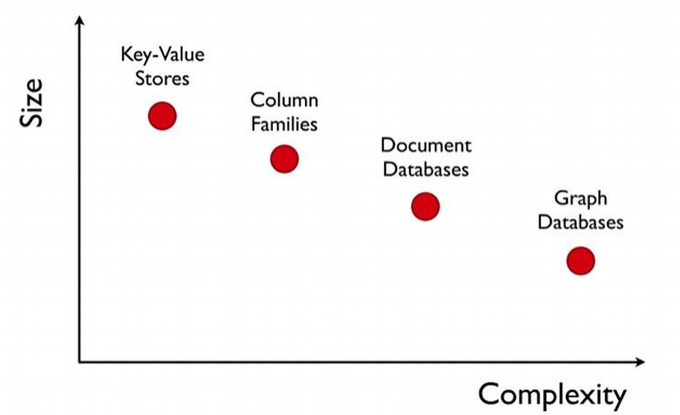
\includegraphics[scale=0.5]{IMAGE1.png}
%	\caption{Processo di Real World Communication Planning}
%	\label{fig:RealWorld}
%\end{figure}

Un'altra agenzia è MEC usa un percorso detto T5 simile al gioco di snake, rappresenta il percorso che un cliente fa. 
Inoltre abbiamo un nastro trasportatore che rappresenta il ciclo tra Trigger e Purchase del cliente nella quale nella fase trigger abbiamo un desiderio, seguito da una fase attiva che porta all'acquisto (stadio purchase), dopo acquisto abbiamo una fase passiva dove il cliente non compra il prodotto.

\subsection{Il Processo di Local Planet nel caso Amplifon}
Local Planet non vede solo i dati che riceve ma va anche ad osservare i clienti a 35 diversi store di amplifon in Europa.
E Tira fuori osservazioni interessanti di similarità e dissimilarità tra i vari paesi. 
Ad esempio, scopre che gli anziani in paesi bassi sono molto indipendenti quindi se mirare loro per vendere i prodotti, mentre nei paesi come Spagna e Italia, dipendono molto dai propri figli quindi ha senso mirare anche i figli per vendere apparecchi acustici per i loro genitori.

Il processo di vendita è molto complesso, contiene anche diverse fasi di testing e appuntamenti personalizzati, il mezzo di pubblicità da usare dipende dal paese. 
Inoltre la fase di awareness è lo step fondamentale per portare il consumatore a considerare l'acquisto di tale prodotto ed è importante il brand building per avere dei clienti fedeli e avvocati della propria marca.

Si possono anche usare tecniche statistiche e di Machine Learning per prevedere future vendite a patto che le condizioni del mercato rimangono più o meno invariate. 
Gli studi statistici possono essere utili per vedere l'efficacia delle pubblicità in varie fasi del giorno e il numero ottimale di pubblicità alla settimana da presentare (Si considera il costo è l'efficacia del canale) che nel caso di amplifon risulta tra 300 e 320.
In caso di mancanza di pubblicità si nota un calo di vendita ripido a differenza anche una settimana.

La fonte dei dati può essere First Party (proprio), Second Party (sfruttando sistemi semantici e i metadati ottenuti da pubblicità) o Third Party. 
Tali dati vengono immagazzinati spesso usando sistemi di Data Lake per poi essere modellati ed elaborati.

\section{Lezione 4 - Attilio - 27 marzo}

Un modello trova relazioni tra variabili che tendenzialmente noi tenderemo ad non considerare. E servono per rispondere alle domande del marketing manager per giustificare le loro azioni.
Il branded content è ad esempio la nissan che sponsorizza le gare sportive estreme oppure red bull che organizza le gare strane estreme ecc.

Uno studio sulle branded content in TV dividendo in 5 gruppi 1500 mamme con figli tra 3 e 16 anni così composti:

\begin{nosepitemize}
	\item 300 che guardano pubblicità di 30 secondi
	\item 300 che guardano pubblicità di 60 secondi
	\item 300 che guardano pubblicità di 90 secondi
	\item 300 a cui viene mostrato il banner
	\item 300 che non vedono niente
\end{nosepitemize}

E si nota che la crescita significativa dell'awareness avviene a 90 secondi, che costa di più  ma si riesce a trasmettere il messaggio in maniera più significativa. 

Un esempio simile è quello della campagna di Volswagen, ottenedo un successo maggiore dopo esposizione della propria marca con pubblicità sui micrositi.
Inoltre si nota in altri studi che lo sponsorship è più effettivo rispetto a spot pubblicitario sulla TV.

Ma ciò non significa che non si investe nella TV, perché l'audience delle sponsorship è limitato, mentre il TV posso espandere l'investimento a piacere raggiungendo praticamente tutta la popolazione.

Il mercato Italiano nel 2017 ha circa la metà occupata dalla TV (pubblicità) mentre circa il 25\% dall'internet e la stampa occupa circa il 12\% ed è stimata una crescita di investimento nel digitale e in decrescita nella stampa.

Il paese in cui crescono gli investimenti più rapidamente è India seguita da Cina e Russia con una buona fetta nell'investimento digitale.
In realtà è un trend mondiale della crescita di investimenti nel digitali com'è giusto aspettarselo, visto l'aumento della popolazione che usa Internet, che può essere visto dal traffico globale dei dati e le Wearable device che aumentano sempre di più. Un altro ambito in aumento in questo momento è il social network.

I paesi occidentali usano molto di più la TV rispetto ai paesi in via di sviluppo, che sembrano preferire il digitale. In Italia il 50\% della fetta pubblicità nella TV è occupata da Gruppo Mediaset seguito da Rai Pubblicità (20\%).

Tante aziende comprano i fan ottendo una grande fan base, ma bisogna capire come usare questi fan, la cosa migiore è usare i social come canali di trasmissioni di messaggio a due via ottenendo feedback dai propri clienti.

\section{Lezione 3 - Di Domenica - 29 marzo}

Google Analytics è un servizio gratuito messo a disposizione da Google ed è il servizio più uitilizzato per le Web Statistics e permette di utilizzare le KPI (Key performing indices) e report e transazioni su un sito Web per conoscere la propria audience, vendere e convertire e agire sugli insights. In realtà esiste una versione commerciale che permette di agire su azioni singole.
\newline
Gli obiettivi (cosa posso fare di Google Analytics):
\begin{nosepitemize}
	\item Conoscere la propria Audience:
	\begin{nosepitemize}
		\item Segmentazione Avanzata: Isolare e analizzare subset di traffico, es. visite che conducono ad una vendita;
		\item Analisi di performance dell'APP;
		\item Audience Data and Reporting: focus specifici sulla Audience;
		\item Dimensioni customizzabili: Focalizzarsi su metriche specifiche (data, attributi demografici, dati comportamentali)
	\end{nosepitemize}
	\item Tenere traccia dei percorsi:
	\begin{nosepitemize}
		\item Flow Visualization: Vedere le pagine visualizzate e percorsi di uscita dell'Audience
		\item Map Overlay: mappe geografiche dei visitatori
		\item Mobile Traffic
		\item Social Reports: l'impatto dei social sul business
		\item Sorgenti di traffico
	\end{nosepitemize}
	\item Comprendere le esigenze
	\begin{nosepitemize}
		\item Event Tracking: Iterazione dell'audience con le pagine;
		\item In-Page Analytics: Iterazione in pagine specifiche
		\item Real-Time Reporting
		\item Site Search
	\end{nosepitemize}
\end{nosepitemize}

Grazie a questi punti posso:
\begin{nosepitemize}
	\item Raggiungere obiettivi di performance: Sfruttando le advertising Reports capisco i risultati per il budget sostenuto, effettuare classificazioni Data-Driven, identificare i prodotti migliori e capire l'impatto di ciascuna azioni di Digital Marketing sulle vendite;
	\item Raggiungere l'Audience corretta: Individuare i consumatori interessati per un prodotto;
	\item Rendere efficiente il sito Web: Alert in variazioni di traffico e capire inefficienze tecninche nel sito.
\end{nosepitemize}

I skills necessari per digitalizzare la mia azienda, sfruttando Google Analytics sono:

\begin{nosepitemize}
	\item Digital marketing e digital advertising
	\item Gestione affiliation and partnership
	\item Creatività grafica e promozionale
	\item Competenze tecniche per sviluppo e gestione del sito
	\item Gestione dei contenuti
	\item Logistica e Operazione per il magazzino
	\item Customer Service
	\item Gestione processo dall'inizio alla fine
	\item Competenze legali e fiscali (per GDPR ecc.)
	\item Skill relazionali e integrazione con altre funzioni aziendali
\end{nosepitemize}

La strategia sui social si basa prima di tutto chiedendosi il perché: che può essere per focalizzarsi sul cliente, massimizzando il coinvolgimento dei clienti e rendendo la customer experience unica e per focalizzarsi sull'azienda, riducendo i costi operativi e aumentando la ROI con le iniziative di marketing e stando attenti alla dispersione dei social media (in divisioni del business e aree geografiche).
Poi segue il come: le domande di solito sono:
\begin{nosepitemize}
	\item come inglobare le funzionalità dei social nelle fuzioni aziendali?
	\item come utilizzare i dati dei canali per la segmentazioni dei clienti?
	\item come catturare la customer voice per sviluppo di prodotti innovativi?
	\item come integrare i social media nelle attività di marketing per ricavare informazioni sui clienti?
\end{nosepitemize}

Gli indicatori principali per comprendere e definire gli investimenti legati al Social CRM sono:
\begin{nosepitemize}
	\item Acquisizioni e Retention dei clienti per aumentare i ricavi
	\item Aumentare la Customer experience per aumentare il coinvolgimento dei clienti aumentando la loro fiducia, loyalty, soddisfazione e awareness
	\item Customer Innovation per ampliare l'innovazione con nuove idee
	\item e in tutte le aree l'azienda vorebbe diminuire i costi e i rischi
\end{nosepitemize}

Le skill necessarie per le varie fasi di Social Media sono: Pianificare, Ascoltare (Monitoro e analizzo), Coinvolgere(con Social media dentro la piattaforma[on board] e fuori dalla piattaforma[off board]) e Ottimizzare la ROI e integrazione CRM aumentando il valore dei Social Media, tutto questo per imparare, Reagire, Supportare, Guidare marketing e sales e infine Servire Cross Channel.

Per sfruttare bene i Social Media (ad es. Twitter) posso: Creare Account Personalizzati per creare una comunità attiva, fare targeting con gli account sponsorizzati che permette di individuare target mirati in base a analogia di follower, parole chiavi nella cronologia, dispositivo usato, sesso, interessi, area geografica ecc. e infine posso usare tattiche promozionali ad esempio usando un approccio creativoper potenziare le vendite o crescere l'awareness del marchio. Attenzione la tattica è diversa da strategia, la strategia è per un periodo lungo mentre le tattiche sono per un periodo breve, quindi sfruttare:
\begin{nosepitemize}
	\item Eventi: settoriali (E3, GamesCom), stagionali (Mother's Day, Capodanno) e culturali (Oscar);
	\item Lancio del Prodotto: Creo Hype, pianificando in anticipo e usando i Social Media e tenere traccia dei risultati ottenuti per amplificarne l'impatto;
	\item Flock  2 Unlock: Usare un incentivo apprezzato creando delle esclusive per Twitter, creando aspettative twittando informazioni specifiche sulla campagna, interagendo con i follower, quando si raggiunge il numero di tweet definito offrire ai follower una ricompensa meritata e mantenere vivo l'interesse con la campagna che ha datto aumentare la visibiltà;
	\item Twixclusive: Offrire ai follower sconti e promozioni, connettersi ai follower ospitando sessione Q\&A, interviste o chat e far saper a tutti la propria gratitudine.
\end{nosepitemize}
Per misurare l'impatto dei Social bisogna:
\begin{nosepitemize}
	\item Definire gli obiettivi e realizzarli
	\item Non avere paura di chiedere cosa pensano dei Tweets e cercare di migliorare dai feedback
	\item Definire delle metriche:
	\begin{nosepitemize}
		\item Aumento del numero dei follower
		\item Qualità e iterazioni dei follower
		\item Copertura: quante persone ritwittano o metteno like
		\item Traffico: numero di utenti che visitano il sito
		\item Conversione: quanti utenti si iscrivono o comprano il servizio
	\end{nosepitemize}
\end{nosepitemize}

Lo stesso vale anche per Facebook, Facebook permette di definire campagna del tipo:
\begin{nosepitemize}
	\item Click to Website
	\item Page Post Engagement
	\item Page Likes
	\item App Installs
	\item App Engagement
	\item Offer Claims
	\item Event Responses
\end{nosepitemize}
Il target è scelto in base a posizioni, età, sesso, interessi precisi, categorie (più ampie dei interessi precisi) a cui sono interessati e connessioni (ad altre pagine ecc.)

Il problema di Facebook è che non esistono delle API con cui posso connettermi con Facebook per avere informazioni sui miei clienti.
Il costo della publicità dipende dalla dimensione del pubblico, si può scegliere un budget giornaliero oppure budget a vita (la vita della campagna se so quanto deve durare), il costo è basta sul numero di views oppure numero di click che sta sempre sotto il budget fissato.

Dai Social media non bisogna avere paura per i feedback poiché forniscono spunti critici immediati all'azienda, bisogna rispondere ai feedback creando iterazione con il cliente che permette di comunicare, conoscere e convincere il cliente, e una volta ottenuti i feedback utilizzarli al meglio diffondendoli all'interno dell'azienda: nel Markiting, Sales, Customer Service e Communication division.

Il Social Media Analytics consiste nel monitoraggio i Social e altri canali iterattivi allo scopo di rilevare menzioni alla marca e nella raccolta dei dati dei dati delle presenze sui social. 
L'obiettivo strategico è gestire e migliorare il posizionamento aziendali sul web ed è uno strumento ideale per Pubblicizzare le attività, ampliare la rete di contatti, interagire e fidelizzare i clienti e effettuare comunicazioni non convenzionali.

Riassumendo le applicazioni principali sono:
\begin{nosepitemize}
	\item la misurazioni del ricnoscimento del Brand tramite KPI
	\item Monitoraggio della reputazioni
	\item Customer Care e Employee Satisfaction
	\item Analisi di contenuti e opinioni nei gruppi
	\item Analisi delle azioni degli utenti (iterazioni e influenze)
	\item Monitoraggio delle discussioni e opinioni dei clienti
\end{nosepitemize} 
e gli obiettivi sono:
\begin{nosepitemize}
	\item Conversione Rate
	\item Aplification Rate
	\item Applause Rate
	\item Conversione Rate
\end{nosepitemize}

Esistono una marea di tool open Source per la gestione di Social Media Analysis: Lithium, Twitter Sentiment, Twitrratr, HootSuite, Blogmeter, Radian ecc.

E gli elementi distintivi sono: la gestione dei Big Data, profondità di analisi e integrazione con strumenti di analisi evoluta, scalabilità, Data Factory, collegamento con i tool di Data Mining e Predictive Modelling.

\section{Lezione 5 - Attilio - 03 aprile}

L'ecosistema Pubblicitario in Europa consiste in:
\begin{itemize}
	\item Agency: Crea, pianifica e gestisce la pubblicità per i propri clienti, e l'evoluzione tecnologica molto simile a come era nel passato, è indipendente dai clienti e fornisce un punto di vista esterno per vedere la vendita dei prodotti dei propri clienti. Non comunicano direttamente con i clienti hanno a disposizione una piattaforma in comune per essere più effficienti possibile. Per gestire la parte digitale si affidano ai trading desk.
	\item Agency Trading Desk: Mettono a disposizione la loro competenza per usare la buying technology. Sono brannche di un azienda più grossa e sono specializzate nello comprare e ottimizzare media e audiences, lavorano per advertisers e agencies, spesso anche in tempo reale su ad exchanges, ad networks e sell side platforms e alle varie tecnologie a cui sono connesse.
	\item Buying Technologies: Connettono l'advertiser con le exchange e scelgono gli spazi che interessano all'advertisor. Prima quando uno comprava uno spazio all'interno di un giornale non aveva la possibilità di scegliere l'audience, tutti quelli che compravano il giornale vedevano la pubblicità, su digitale abbiamo un sacco di nuove informazioni sull'audience (es. info socio-demografiche e comportamentali dai cookie), le informazioni sono ricevute grazie ai data providers and technologies.
	\item Data Providers and Technologies: Collezionano, compilano e vendono dati anonimi a un cliente, inoltre gestiscono, protteggono e collezioni informazioni da fonti diversi sia online che offline trasformandole in informazione su cui i buying e selling technologies possono agire. Spesso sono anche i delivery systems, tools, analytics, verification and privacy. es. Sizmek e Google
	\item Delivery Systems, Tools, Analytics, Verification and Privacy: Leggono con la loro tecnologia cosa vi piace e nello spazio pubblicitario propongono contenuti che potrebbe interessarvi. Assicurano inoltre che diversi tipi di pubblicità vengano serviti, misurati e validati giustamente e offrono sicurezza e privacy ai advertisers e content provider.
	\item Exchanges: E' dove le piattaforme delle Agency e i marketplace si incontrano per connetere la supply con la domanda, su un certo sito ci sono degli spazi (banner, spazio pubblicitario) es. Google, Amazon
	\item Sales Houses and Ad Networks: Aiutano/Garantisce ad avere maggior fatturato, hanno spesso diversi campi di specializzazione (mobile, retargeting ecc.) e aiutano i content provider, agenzie e advertiser a promuovere i loro spazi nel mercato usando la loro connessione nei campi anche specifici per promuovere il servizio nel posto giusto. I Sales House lavorano spesso in maniera esclusiva per i content provider sia per pubblicità standard che customizzato e fanno i modo che la pubblicità sia vista e costruita nel modo giusto e massimizzi la resa.
	\item Selling Technologies: automatizzano le vendite online in tempo reale e massimizzano i loro revenue, offrono inoltre metodi efficienti, automatici e sicuri per vedere le diverse sorgenti di domanda disponibili e offrono ingsights nei vari revenue streams e audiencies.
	\item Independent Agencies: sono strutture che fanno più o meno le stesse cose dei Trading Desk ma non fanno parte dei gruppi più grandi, ciò sono specializzate nello comprare, ottimizzare media e audiences, lavorano per advertisers e agencies, spesso anche in tempo reale su ad exchanges, ad networks e sell side platforms e alle varie tecnologie a cui sono connesse.
\end{itemize}

\section{Lezione 4 - Di Domenica - 05 aprile}

L'azienda vuole aumentare il valore e la soddisfazione del cliente proponendo la migliore azione durante ogni iterazione. I bisogni dei clienti sono:
\begin{nosepitemize}
	\item Interagire con Social Media
	\item Avere un Contact Centre migliore
	\item Utilizzare i canali Internet
	\item Migliorare i servizi Negozio
	\item Avere indipendenza con Self-service
\end{nosepitemize}
Mentre gli obiettivi del business sono:
\begin{nosepitemize}
	\item Attaccamento al marchio
	\item Aumentare le vendite
	\item Migliorare il caring verso il cliente
	\item Mantenere il cliente senza che mi abbandoni
	\item Raccogliere nuove informazione
	\item Migliorare la conoscenza del cliente
\end{nosepitemize}
C'è bisogno di un naturale bilanciamento tra i bisogni dei clienti e obiettivi del business.

Riusando uno dei modelli precendenti ho che ottenuti i dati necessari ottengo informazione necessaria per la next best action, una volta capito questo ho il design, disegnando, attraverso interfaccia grafica in modilità workflow, le logiche decisionali e impostare le decisioni basate sia su business rules che su processi analitici fatto in Real Time.
Poi definisco delle logiche di prioritizzazione tra le azioni concorrenti, cioè quali azioni proporre al clienti in caso di sovrapposizioni,
segue l'esecuzione in RT (Real Time) le logiche decisionali, integrare con altre applicazioni per raccogliere dati aggiuntivi e per comunicare della decisione.
Infine c'è il controllo e monitoraggio attraverso report multidimensionali.

Per determinare l'offerta più appropriata l'utente può utilizzare informazioni su:
\begin{nosepitemize}
	\item Il comportamento corrente sul sito
	\item Il comportamento storico sul sito
	\item Tutti i canali di contatto preferiti
	\item I modelli predittivi per capirne il comportamento
	\item Valutazione ed arbitraggio tra più offerte
	\item Le regole del Business
\end{nosepitemize}

Un esempio: Il cliente naviga sul sito e in base di navigazione genera in trigger e il trigger fa partire le azioni e al cliente viene presentata una landing page personalizzata.
Inolre sul sito si può determinare il pricing dinamico, determinzione della posizione creditizia online per la preaccettazione di richiesta di prestito/mutuo. \newline
Un altro esempio è un'applicazione all'interno di uno store dove il cliente riceve un alert sul telofono con un'offerta mirata grazie alla valutazione della posizione del cliente, il suo profilo e eventuale informazione del suo carello in RT. Aggiornamento RT può essere effettuato su tutti i canali abilitati ai Web services.

Il CRM nel Social Marketing è così composto:
\begin{nosepitemize}
	\item social media
	\item Altri canali di ingaggio (sia online che offline)
	\item Il sito web
	\item Sale Transaction, che sono i dati offline che possiedo
\end{nosepitemize}
Posso utilizzare questi dati per analizzare l'influenza e le reazioni tra le transazione e come mi comporto sul web, analizzare il sentiment sui prodotti e servizi e infine posso fare Contextual Marketing (possibilmente in RT). Una volta eseguiti questi modelli posso fare data mining analitico, reporting e previsioni. 

Il Real Time Decision manager consente nel comunicare in RT decisioni e proposte commerciali, basate su regole di business e conoscenza analistiche, che guidano ogni interazione con il cliente per aumentarne il profitto, crescita e fidelizzazione.

Le caratteristiche principali sono:
\begin{nosepitemize}
	\item Interfaccia grafica che consente di creare i flussi decisionali in modo semplice ed intuitivo
	\item Interfaccia web service standard per integrazione con tutti i canali (per i modelli predittivi ecc.)
	\item Consente di eseguire lo scoring dei modelli in RT
	\item Tutto in un'architettura scalabile che consente di distribuireun volume considerevole di decisioni alle applicazioni di front-end
\end{nosepitemize}
Un esempio di funzionamento delle interazione in RT:
\begin{enumerate}[noitemsep,topsep=0ex]
	\item Il Frontend/canale richiede una decisione in RT sui dati del cliente
	\item Viene mandata una richiesta via web service al RT decision manager dove
	\item Il RT Decision Manager esegue un processo decisionale con eventuale scoring on line usando il Database già esistente e RT data appena ricevuto
	\item Restituisce la decisione/azione
	\item La decisione viene rinviata alla applicazione Frontend via web service
	\item L'applicazione riceve la decisione e esegue la proposta sul momento
\end{enumerate} 

Il flusso decisionale è costituito:
\begin{nosepitemize}
	\item Start Node: es. sul sito web viene compilato il form per la richiesta di un prestito
	\item Estraggo le informazione finanziarie aggiornate del cliente con un altro nodo
	\item si verifica se il cliente è esistente o nuovo e si procede in base a questa informazione
	\item Un nodo che ricalcola il modello la propensione del rischio del cliente
	\item Definsico con un nodo alcune classi di rischio mandando la richiesta (freccia) a un nodo basato sul rischio
	\item infinte la risposta viene inviata al canale e viene aggiornato lo storico dei contatti
\end{nosepitemize}
Questo modello può prevedere l'implementazione delle regole del business relative ai clienti, determinazione dell'azione da fare sui clienti attraverso il canale, utilizzare i modelli predittivi e integrazione con altri sistemi es. web site.

\section{Lezione 5 - Di Domenica - 12 aprile}



\end{document}